\subsection{Der Klein-Gordon-Propagator}
	\begin{align*}
		\braket{0 | [\phi(x), \phi(y)] | 0} &= 
		\int \frac{\diff^3 p}{(2 \pi)^3} \frac{1}{2 E_p} (e^{-i p(x- y)} - e^{ip (y-x)}) \\
		&= \int \frac{\diff^3 p}{(2 \pi)^3}  
		\left[
			 \left. \frac{1}{2 E_p} e^{-ip(x-y)} \right|_{p^0 = E_p}
			 + \left.  \frac{1}{- 2 E_p} e^{ip(x-y)} \right|_{p^0 = -E_p}
		\right] \\
		&\overset{x^0 > y^0}{=}
		\int \frac{\diff^3 p}{(2 \pi)^3} \frac{\diff p^0}{2 \pi i}
		\frac{-1}{p^2 -m^2} e^{-ip(x-y)} \\
		&\coloneqq D_R (x-y) = \theta(x^0 -y^0) 
		\braket{0 | [\phi(x), \phi(y)] | 0}
	\end{align*}

	\begin{figure} [h]
		\begin{center}
			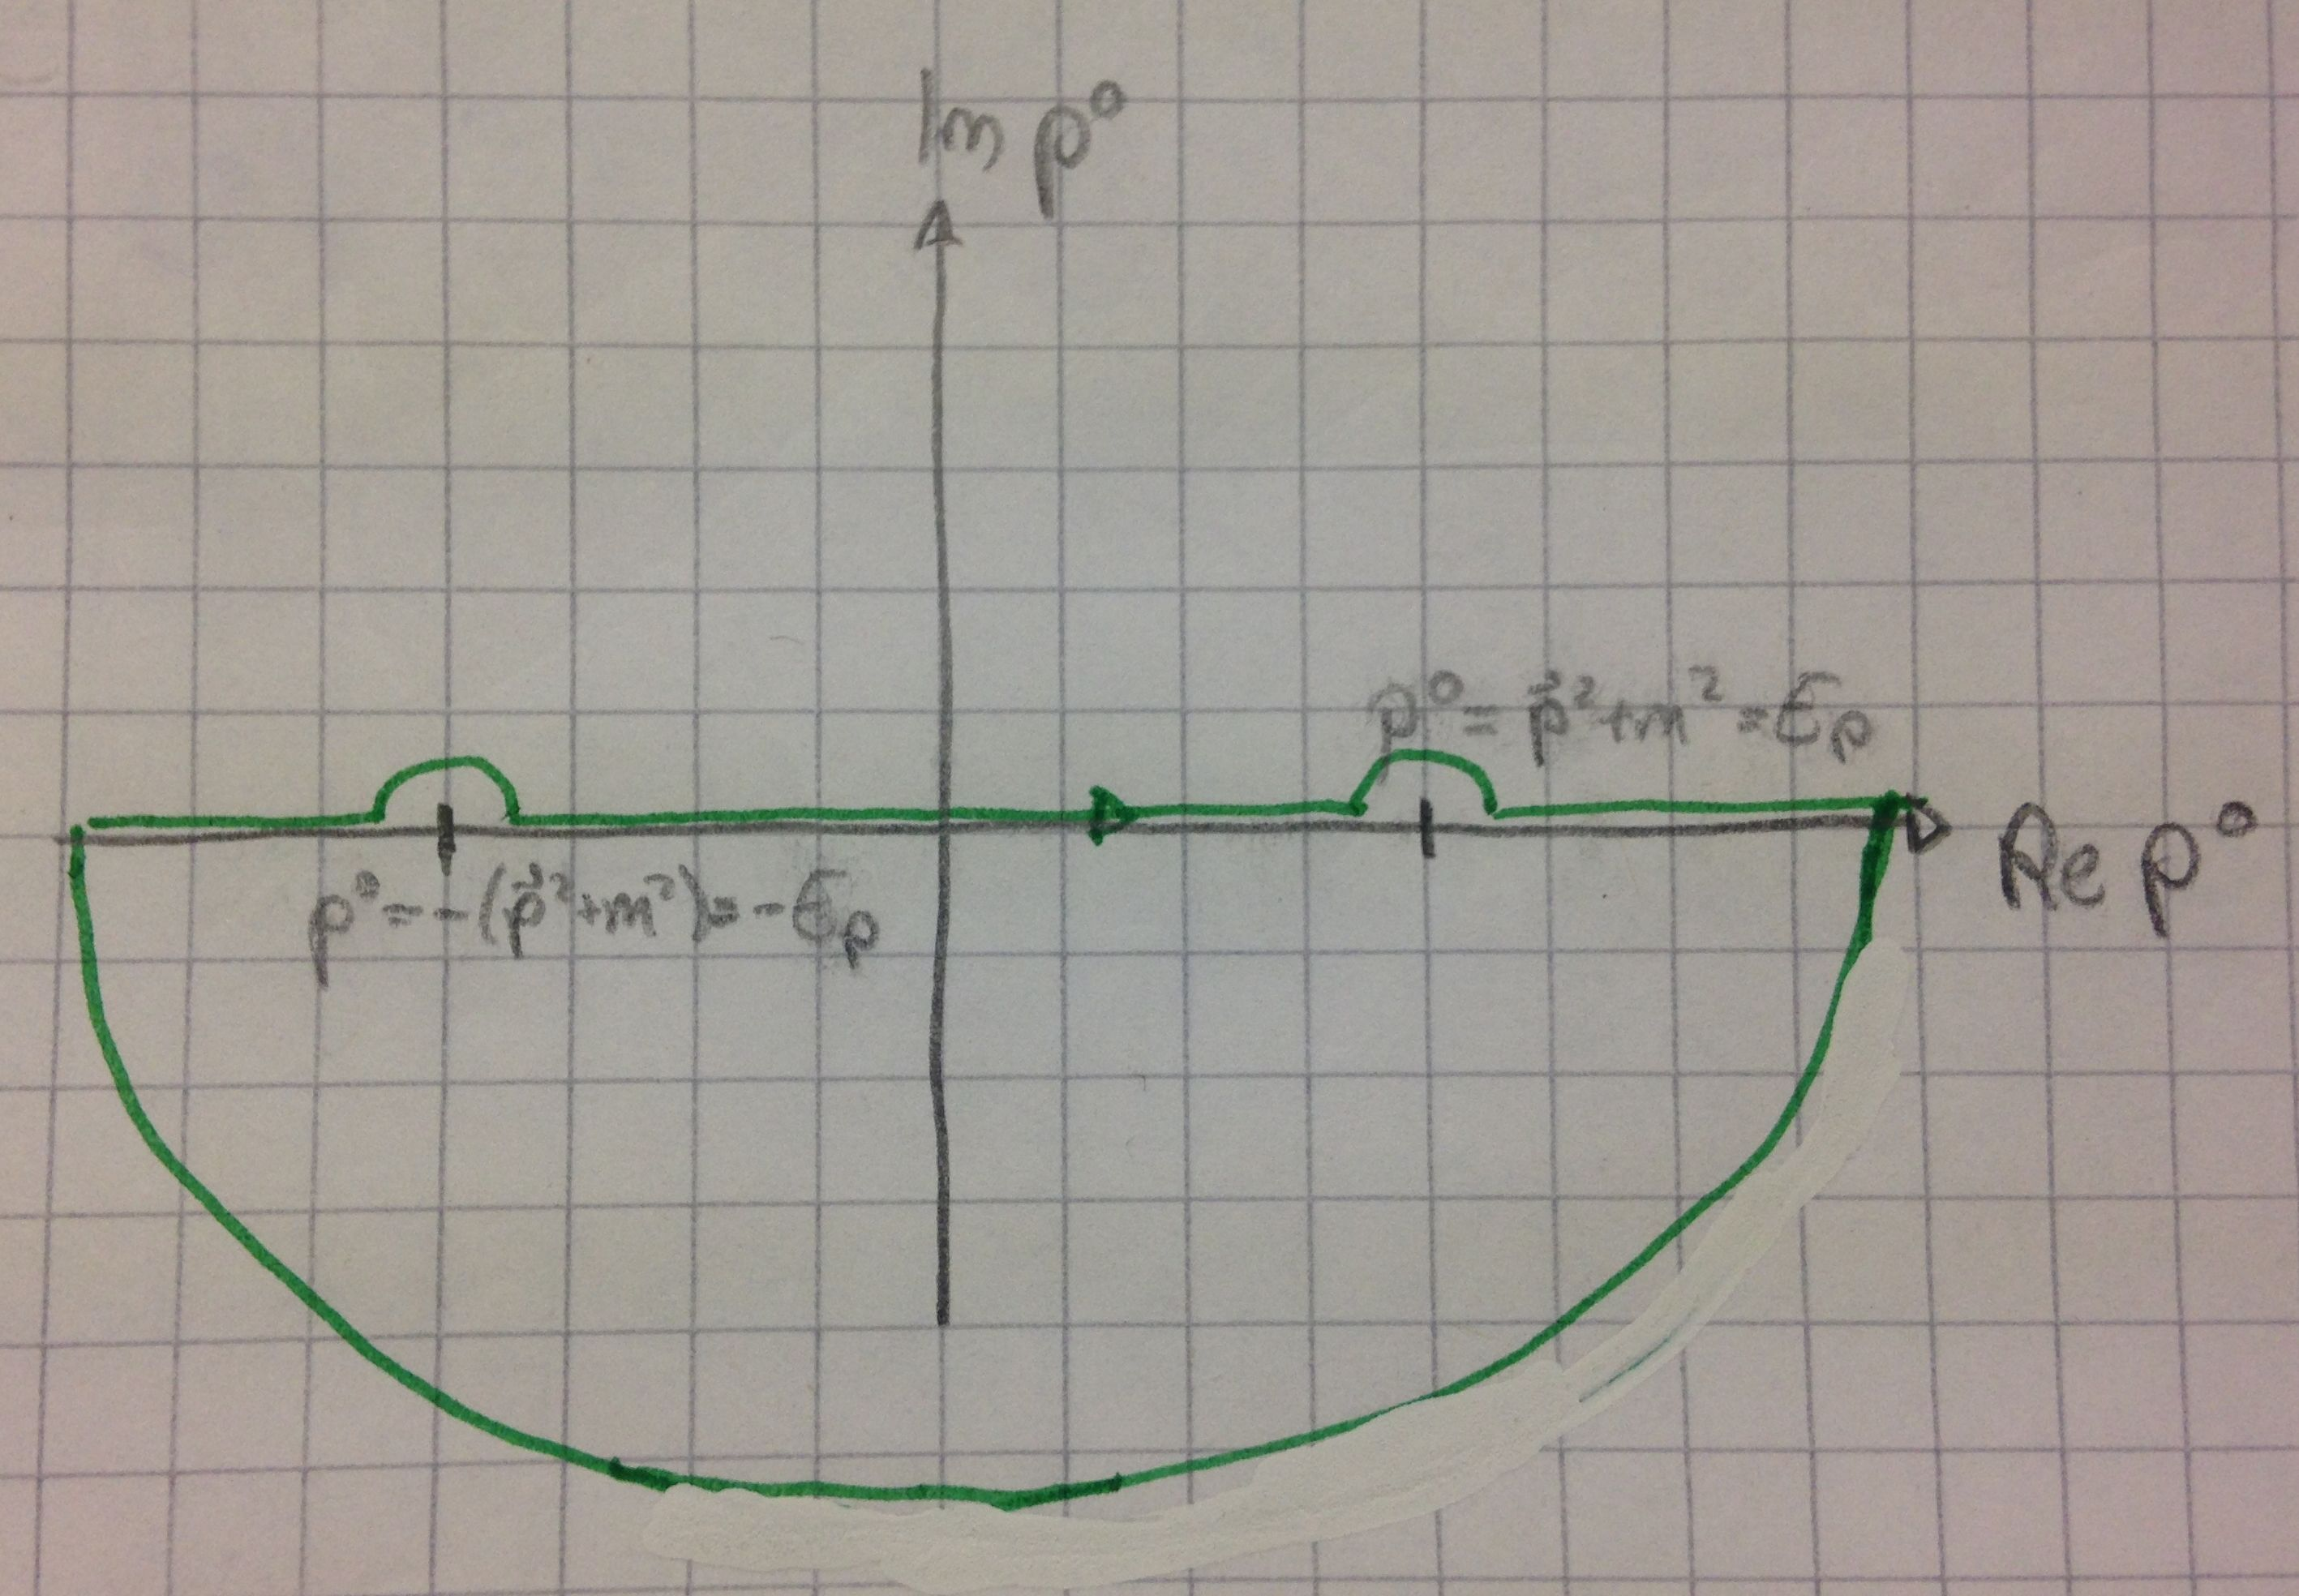
\includegraphics[width = 10cm]{Klein-Gordon-Propagator}
		\end{center}	
	\end{figure}
\FloatBarrier
Beh: $D_R(x-y)$ ist retardierte Greenfunktion des K.G. Operators.
	\begin{align*}
		(\square + m^2) D_R(x-y) &= ? &
		D_R(x-y) &= \int \frac{\diff^4 p}{(2 \pi)^4} e^{-ip(x-y)} \tilde{D}_R (p) \\
		\tilde{D}_R(p) &= \frac{i}{p^2 - m^2} & 
		(-p^2 + m^2) \tilde{D}_R(p) &= -i
	\end{align*}
$\Rightarrow (\square + m^2) D_R(x-y) = -i \delta^{(4)} (x-y)$

Alternativ
	\begin{align*}
		& (\square + m^2)\braket{0 | [\phi(x), \phi(y)] | 0} \theta(x^0 - y^0) \\
		&=
		\left(
			\partial_\mu \partial^\mu \theta(x^0 - y^0) \braket{0 | [\phi(x), \phi(y)] | 0} + 2 \partial_\mu \theta \braket{0 | [\partial^\mu \phi(x), \phi(y)] | 0}
		\right) \\
		&+ \theta(x^0 - y^0) (\square + m^2) \braket{0 | [\phi(x), \phi(y)] | 0} \\
		&= \partial_0 (\theta(x^0 -y^0)) \braket{0 | [\partial^0 \phi(x), \phi(y)] | 0} \\
		&= \delta(x^0 -y^0) \braket{0 | [\pi(x), \phi(y)] | 0} = -i \delta^{(4)}(x-y) \checkmark
	\end{align*} 
WdH: \marginpar{01.02.16}

$[\phi(y), \phi(x)] \ket{n} = D(x- y) - D(y -x)$ 

Letzte Vorlesung Zeichnung, wenn durch die Mitte geht, dann kann man das nicht einfach überführen. 

$D(y -x) = D(x -y)$ nur für raumartige.

für avancierte Funktion wäre $x^0 < y^0$ gewesen, wir hätten obenrum integrieren müssen. 
\\ \\
4 verschiedene ``Integrationsmöglichkeiten'', festgelegt durch Vorzeichen von $x^0 - y^0$, relativ zu $p^0$.

Interessante (neue) Möglichkeit: \underline{Feynmanpropagator:}
	\begin{align*}
		\boxed{D_F(x -y) = \int \frac{\diff^4 p}{(2 \pi)^4} \frac{i}{p^2 -m^2 + i\epsilon} e^{-ip(x-y)} }
	\end{align*}
Pole bei $p_0 = \pm \sqrt{\vec{p}^2 + m^2 - i\epsilon} = \pm \sqrt{\vec{p}^2 + m^2}\left(1 -\frac{i}{2} \epsilon\right) = \pm \sqrt{\vec{p}^2 + m^2} \mp i \epsilon'$

Nur zur Erinnerung, $p_0$ ist die Energiekomponente des Viererimpulses.

	\begin{figure} [h]
		\begin{center}
			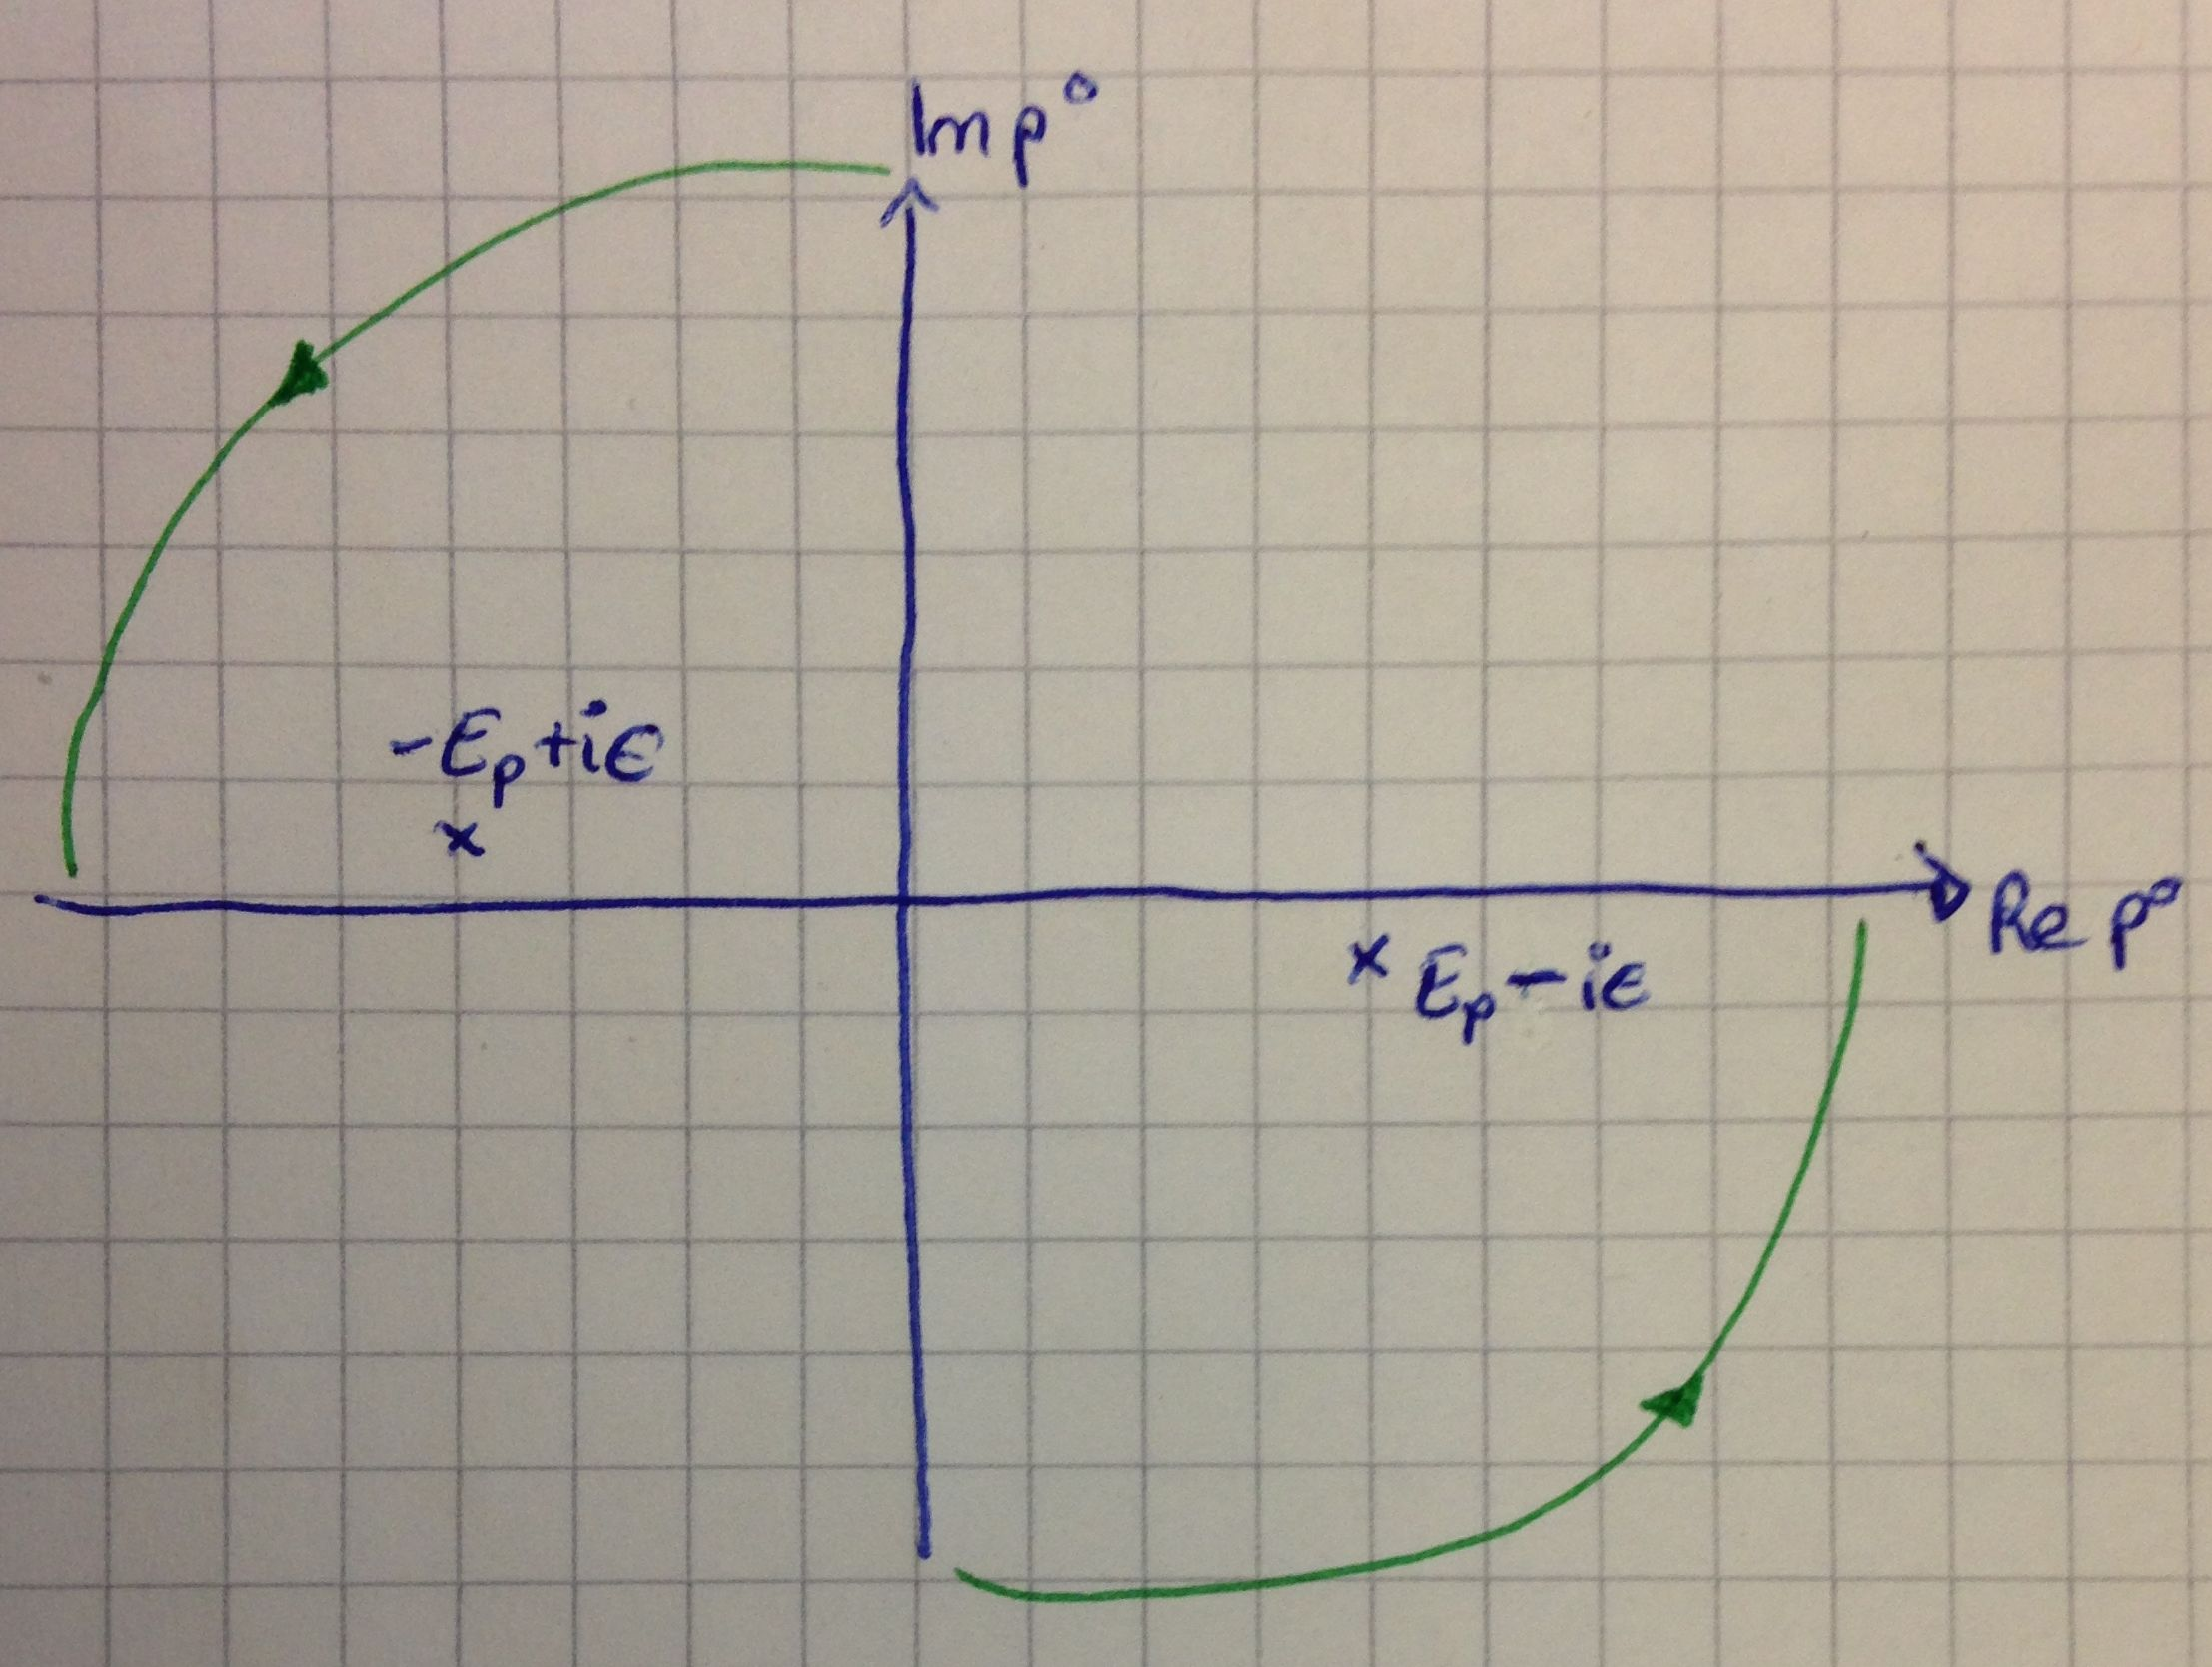
\includegraphics[width = 10cm]{Klein-Gordon-Propagator2}
		\end{center}	
	\end{figure}

	\begin{tabular}{l l l}
		$x^0 < y^0$ (avancierte Lösung) &:& $e^{-i \ldots} \rightarrow 0$ für Im $p^0>0$\\
		$x^0 > y^0$ (retardierte Lösung) &:& $e^{-i \ldots} \rightarrow 0$ für Im $p^0 <0$
 	\end{tabular}
 	\begin{align*}
	 	D_F(x-y) &=
	 	\left\{
	 	\begin{aligned}
		 	D(x-y) &\text{ für } x^0 > y^0 \\
		 	D(y-x) &\text{ für } x^0 < y^0 
	 	\end{aligned}
	 	\right. \\
	 	&= \theta (x^0- y^0) \braket{0 | \phi (x) \phi(y) | 0} + 
	 	\theta(y^0 -x^0) \braket{0 | \phi (y) \phi(x) | 0}
 	\end{align*}
 	\begin{align*}
	 	\boxed{D_F(x-y) = \braket{0 | \mathrm{T}\phi (x) \phi(y) | 0}}
 	\end{align*}
 T steht für die Zeitordnung.
 
 Feynmanvorschrift entspricht Erwartungswerten zeitgeordneter Operatoren. 
 \\
 Lösung der K-G-Gleichung für eine klassische Quelle:
	 \begin{align*}
		 (\square + m^2) \phi(x) = j(x)
	 \end{align*}
ist die Bewegungsgleichung für 
	\begin{align*}
		\La &= \frac{1}{2} (\partial_\mu \phi) (\partial^\mu \phi) - \frac{1}{2} m^2 \phi^2 + j(x) \phi(x)
	\end{align*}
Massendimenstion von $\phi$: 1 ($m^1$), $j$: 3 ($m^3$)

Annahme $j(x) \neq 0$ für endliches Zeitintervall.

Vor Einschalten von $j(x)$ (Strom)
	\begin{align*}
		\phi_0 &= \int \frac{\diff^3 p}{(2\pi)^3} \frac{1}{\sqrt{2 E_p}} 
		\left(
			a_{\vec{p}} e^{-ipx} - a_{\vec{p}}^\dagger e^{-ipx}
		\right)
	\end{align*}
für $x^0 > y^0$: (das $i$ vor dem $\int$ kommt von: $i(\square+m^2)D_R = i\delta$ setzen)
	\begin{align*}
		\phi(x) &= \phi_0(x) + i\int \diff^4 y D_R (x- y) j(y) \\
		&= \phi_0 (x) + i \int \diff^4 y 
		\overbrace{\int\frac{\diff^4 p}{(2 \pi)^4} \delta(p^2 -m^2)\theta(x^0 - y^0)}^{\mathclap{\int \frac{\diff^3 p}{(2\pi)^4} \frac{1}{2 E_p}}}
		\left( \vphantom{e^{-ip(x-y)} - e^{ip(x-y)}} \right.
			\overbrace{e^{-ip(x-y)}}^{\mathclap{\tilde{j}(p)}} 
			- \underbrace{e^{ip(x-y)}}_{\mathclap{\tilde{j}^*(p)= \tilde{j}(-p) \text{ weil } j \text{ reell}}}
		\left. \vphantom{e^{-ip(x-y)} - e^{ip(x-y)}} \right)j(y)
	\end{align*}
	\begin{align*}
		\phi(x) &= \int \frac{\diff^3 p}{(2\pi)^3} \frac{1}{2 E_p}
		\left\{
			\left(
				a_{\vec{p}} + \frac{i}{\sqrt{2 E_p}} \tilde{j}(p) 
			\right)e^{-ipx}
			+
			\left(
				a_{\vec{p}}^\dagger - \frac{i}{\sqrt{2 E_p}} \tilde{j}^*(p) 
			\right)e^{ipx}
		\right\} \\
		\Rightarrow H &= \int \frac{\diff^3 p}{(2 \pi)^3} E_p 
		\left(
			a_{\vec{p}}^\dagger - \frac{i}{\sqrt{2 E_p}} \tilde{j}^*(p) 
		\right)
		\left(
		a_{\vec{p}} + \frac{i}{\sqrt{2 E_p}} \tilde{j}(p) 
		\right)
		+ \text{ ``Nullpunktsenergie''}
	\end{align*}
(Gleiche Rechnung wie vorher)

Energie für $x^0 > y^0$:
	\begin{align*}
		\boxed{
				\braket{0 | H | 0} =
				\int \frac{\diff^3 p}{(2 \pi)^3} E_p \frac{1}{2E_p} | \tilde{j}(p)|^2 
				= \int \frac{\diff^3 p}{(2 \pi)^3} \frac{1}{2} | \tilde{j}(p)|^2  
			}
	\end{align*}
Energie, die durch Strom dem System zugeführt wird

$\Rightarrow$ Feld hat Energie
	
$\Rightarrow j$ erzeugt Feld/Teilchen

Anzahl:
	\begin{align*}
		N = \int \frac{\diff^3 p}{(2 \pi)^3} \overbrace{\frac{1}{2E_p} | \tilde{j}(p)|^2}^{\mathclap{N_{\vec{p}}}}
	\end{align*}
$\frac{1}{2E_p} | \tilde{j}(p)|^2$ Wahrscheinlichkeitsdichte eines Teilchens/Mode $\vec{p}$ zu erzeugen.